%%%%%%%%%%%%%%%%%%%%%%%%%%%%%%%%%%%%%%%%%%%%%%%%%%%%%%%%%%%%%%%%%%%%%
%% This is a (brief) model paper using the achemso class
%% The document class accepts keyval options, which should include
%% the target journal and optionally the manuscript type. 
%%%%%%%%%%%%%%%%%%%%%%%%%%%%%%%%%%%%%%%%%%%%%%%%%%%%%%%%%%%%%%%%%%%%%
\documentclass[journal=jceda8,manuscript=article]{achemso}

%%%%%%%%%%%%%%%%%%%%%%%%%%%%%%%%%%%%%%%%%%%%%%%%%%%%%%%%%%%%%%%%%%%%%
%% Place any additional packages needed here.  Only include packages
%% which are essential, to avoid problems later. Do NOT use any
%% packages which require e-TeX (for example etoolbox): the e-TeX
%% extensions are not currently available on the ACS conversion
%% servers.
%%%%%%%%%%%%%%%%%%%%%%%%%%%%%%%%%%%%%%%%%%%%%%%%%%%%%%%%%%%%%%%%%%%%%
\usepackage[version=3]{mhchem} % Formula subscripts using \ce{}
\usepackage{hyperref}
%%%%%%%%%%%%%%%%%%%%%%%%%%%%%%%%%%%%%%%%%%%%%%%%%%%%%%%%%%%%%%%%%%%%%
%% If issues arise when submitting your manuscript, you may want to
%% un-comment the next line.  This provides information on the
%% version of every file you have used.
%%%%%%%%%%%%%%%%%%%%%%%%%%%%%%%%%%%%%%%%%%%%%%%%%%%%%%%%%%%%%%%%%%%%%
%%\listfiles

%%%%%%%%%%%%%%%%%%%%%%%%%%%%%%%%%%%%%%%%%%%%%%%%%%%%%%%%%%%%%%%%%%%%%
%% Place any additional macros here.  Please use \newcommand* where
%% possible, and avoid layout-changing macros (which are not used
%% when typesetting).
%%%%%%%%%%%%%%%%%%%%%%%%%%%%%%%%%%%%%%%%%%%%%%%%%%%%%%%%%%%%%%%%%%%%%
\newcommand*\mycommand[1]{\texttt{\emph{#1}}}

%%%%%%%%%%%%%%%%%%%%%%%%%%%%%%%%%%%%%%%%%%%%%%%%%%%%%%%%%%%%%%%%%%%%%
%% Meta-data block
%% ---------------
%% Each author should be given as a separate \author command.
%%
%% Corresponding authors should have an e-mail given after the author
%% name as an \email command. Phone and fax numbers can be given
%% using \phone and \fax, respectively; this information is optional.
%%
%% The affiliation of authors is given after the authors; each
%% \affiliation command applies to all preceding authors not already
%% assigned an affiliation.
%%
%% The affiliation takes an option argument for the short name.  This
%% will typically be something like "University of Somewhere".
%%
%% The \altaffiliation macro should be used for new address, etc.
%% On the other hand, \alsoaffiliation is used on a per author basis
%% when authors are associated with multiple institutions.
%%%%%%%%%%%%%%%%%%%%%%%%%%%%%%%%%%%%%%%%%%%%%%%%%%%%%%%%%%%%%%%%%%%%%
\author{Peng Liu}
\affiliation[Pitt]{Department of Chemistry, University of Pittsburgh}
\author{David R. Koes}
\email{dkoes@pitt.edu}
\affiliation[Pitt]{Department of Computational and Systems Biology, University of Pittsburgh}

%%%%%%%%%%%%%%%%%%%%%%%%%%%%%%%%%%%%%%%%%%%%%%%%%%%%%%%%%%%%%%%%%%%%%
%% The document title should be given as usual. Some journals require
%% a running title from the author: this should be supplied as an
%% optional argument to \title.
%%%%%%%%%%%%%%%%%%%%%%%%%%%%%%%%%%%%%%%%%%%%%%%%%%%%%%%%%%%%%%%%%%%%%
\title[3Dmol.js]
  {The 3Dmol.js classroom response system for 3D chemical structures}

%%%%%%%%%%%%%%%%%%%%%%%%%%%%%%%%%%%%%%%%%%%%%%%%%%%%%%%%%%%%%%%%%%%%%
%% Some journals require a list of abbreviations or keywords to be
%% supplied. These should be set up here, and will be printed after
%% the title and author information, if needed.
%%%%%%%%%%%%%%%%%%%%%%%%%%%%%%%%%%%%%%%%%%%%%%%%%%%%%%%%%%%%%%%%%%%%%
\keywords{audience response system, clickers, active learning}

%%%%%%%%%%%%%%%%%%%%%%%%%%%%%%%%%%%%%%%%%%%%%%%%%%%%%%%%%%%%%%%%%%%%%
%% The manuscript does not need to include \maketitle, which is
%% executed automatically.
%%%%%%%%%%%%%%%%%%%%%%%%%%%%%%%%%%%%%%%%%%%%%%%%%%%%%%%%%%%%%%%%%%%%%
\begin{document}

%%%%%%%%%%%%%%%%%%%%%%%%%%%%%%%%%%%%%%%%%%%%%%%%%%%%%%%%%%%%%%%%%%%%%
%% The "tocentry" environment can be used to create an entry for the
%% graphical table of contents. It is given here as some journals
%% require that it is printed as part of the abstract page. It will
%% be automatically moved as appropriate.
%%%%%%%%%%%%%%%%%%%%%%%%%%%%%%%%%%%%%%%%%%%%%%%%%%%%%%%%%%%%%%%%%%%%%
\begin{tocentry}
\end{tocentry}

%%%%%%%%%%%%%%%%%%%%%%%%%%%%%%%%%%%%%%%%%%%%%%%%%%%%%%%%%%%%%%%%%%%%%
%% The abstract environment will automatically gobble the contents
%% if an abstract is not used by the target journal.
%%%%%%%%%%%%%%%%%%%%%%%%%%%%%%%%%%%%%%%%%%%%%%%%%%%%%%%%%%%%%%%%%%%%%
\begin{abstract}
Classroom response systems are an important tool in many active learning pedagogies.  They support real-time feedback on student learning and promote student engagement, even in large classrooms, by allowing instructors to solicit an answer to a question from all students and show the results. Existing classroom response systems are general purpose and not tailored to the specific needs of a chemistry classroom.  In particular, it is not easy to deploy molecular representations except as static images. Here we present a classroom response system that uses the open source web-based 3Dmol.js JavaScript framework to provide interactive viewing and querying of 3D molecules and provide a case study of its use in an organic chemistry recitation.
\end{abstract}

%%%%%%%%%%%%%%%%%%%%%%%%%%%%%%%%%%%%%%%%%%%%%%%%%%%%%%%%%%%%%%%%%%%%%
%% Start the main part of the manuscript here.
%%%%%%%%%%%%%%%%%%%%%%%%%%%%%%%%%%%%%%%%%%%%%%%%%%%%%%%%%%%%%%%%%%%%%
\section{Introduction}
Active learning is ``the process of having students engage in some activity that forces them to reflect upon ideas and how they are using those ideas''\cite{collins2011greenwood}.  The application of active learning pedagogies results in significant improvements in learning outcomes in science classrooms\cite{michael2006s,deslauriers2011improved,armbruster2009active}, including organic chemistry classes\cite{jeske2019collaborative,decicco2019clickers,webbased}.  One popular active learning method is the use of classroom response systems\cite{martyn2007clickers}, also known as audience/student/personal response systems or ``clickers.''  In these systems, the instructor poses a question and students answer using a personal device, either a dedicate piece of hardware (a ``clicker'') or a web-enabled device such as a smartphone or laptop\cite{webbased}.  Students answer anonymously and the collated answers are shown to the class to enable further discussion.  In a meta-analysis\cite{hunsu2016meta} of 53 studies, the use classroom response systems, by themselves without the inclusion of any other active learning methodology, was found to produce a small, but statistically significant, benefit on cognitive outcomes and a larger benefit on non-cognitive outcomes, such as the students' enjoyment of the class and ranking of the instructor.

The use of classroom response systems in the chemistry classroom is growing, particular for large classes\cite{gibbons2017chasm,woelk2008optimizing}.  However, general-purpose software not designed specifically for chemistry is often used, reducing the efficacy of the system\cite{webbased}.  Importantly, we are not aware of any system that seamlessly integrates 3D chemical structures, which are important for engaging students and enabling spatial learning\cite{viz32class}.  To address this need, we have extended the 3Dmol.js\cite{rego20153dmol} JavaScript library for online molecular visualization to include a learning environment with classroom response system features.  We next describe how these features work, provide a case study of their application in an organic chemistry recitation, and discuss future directions.

\begin{figure}
    \centering
    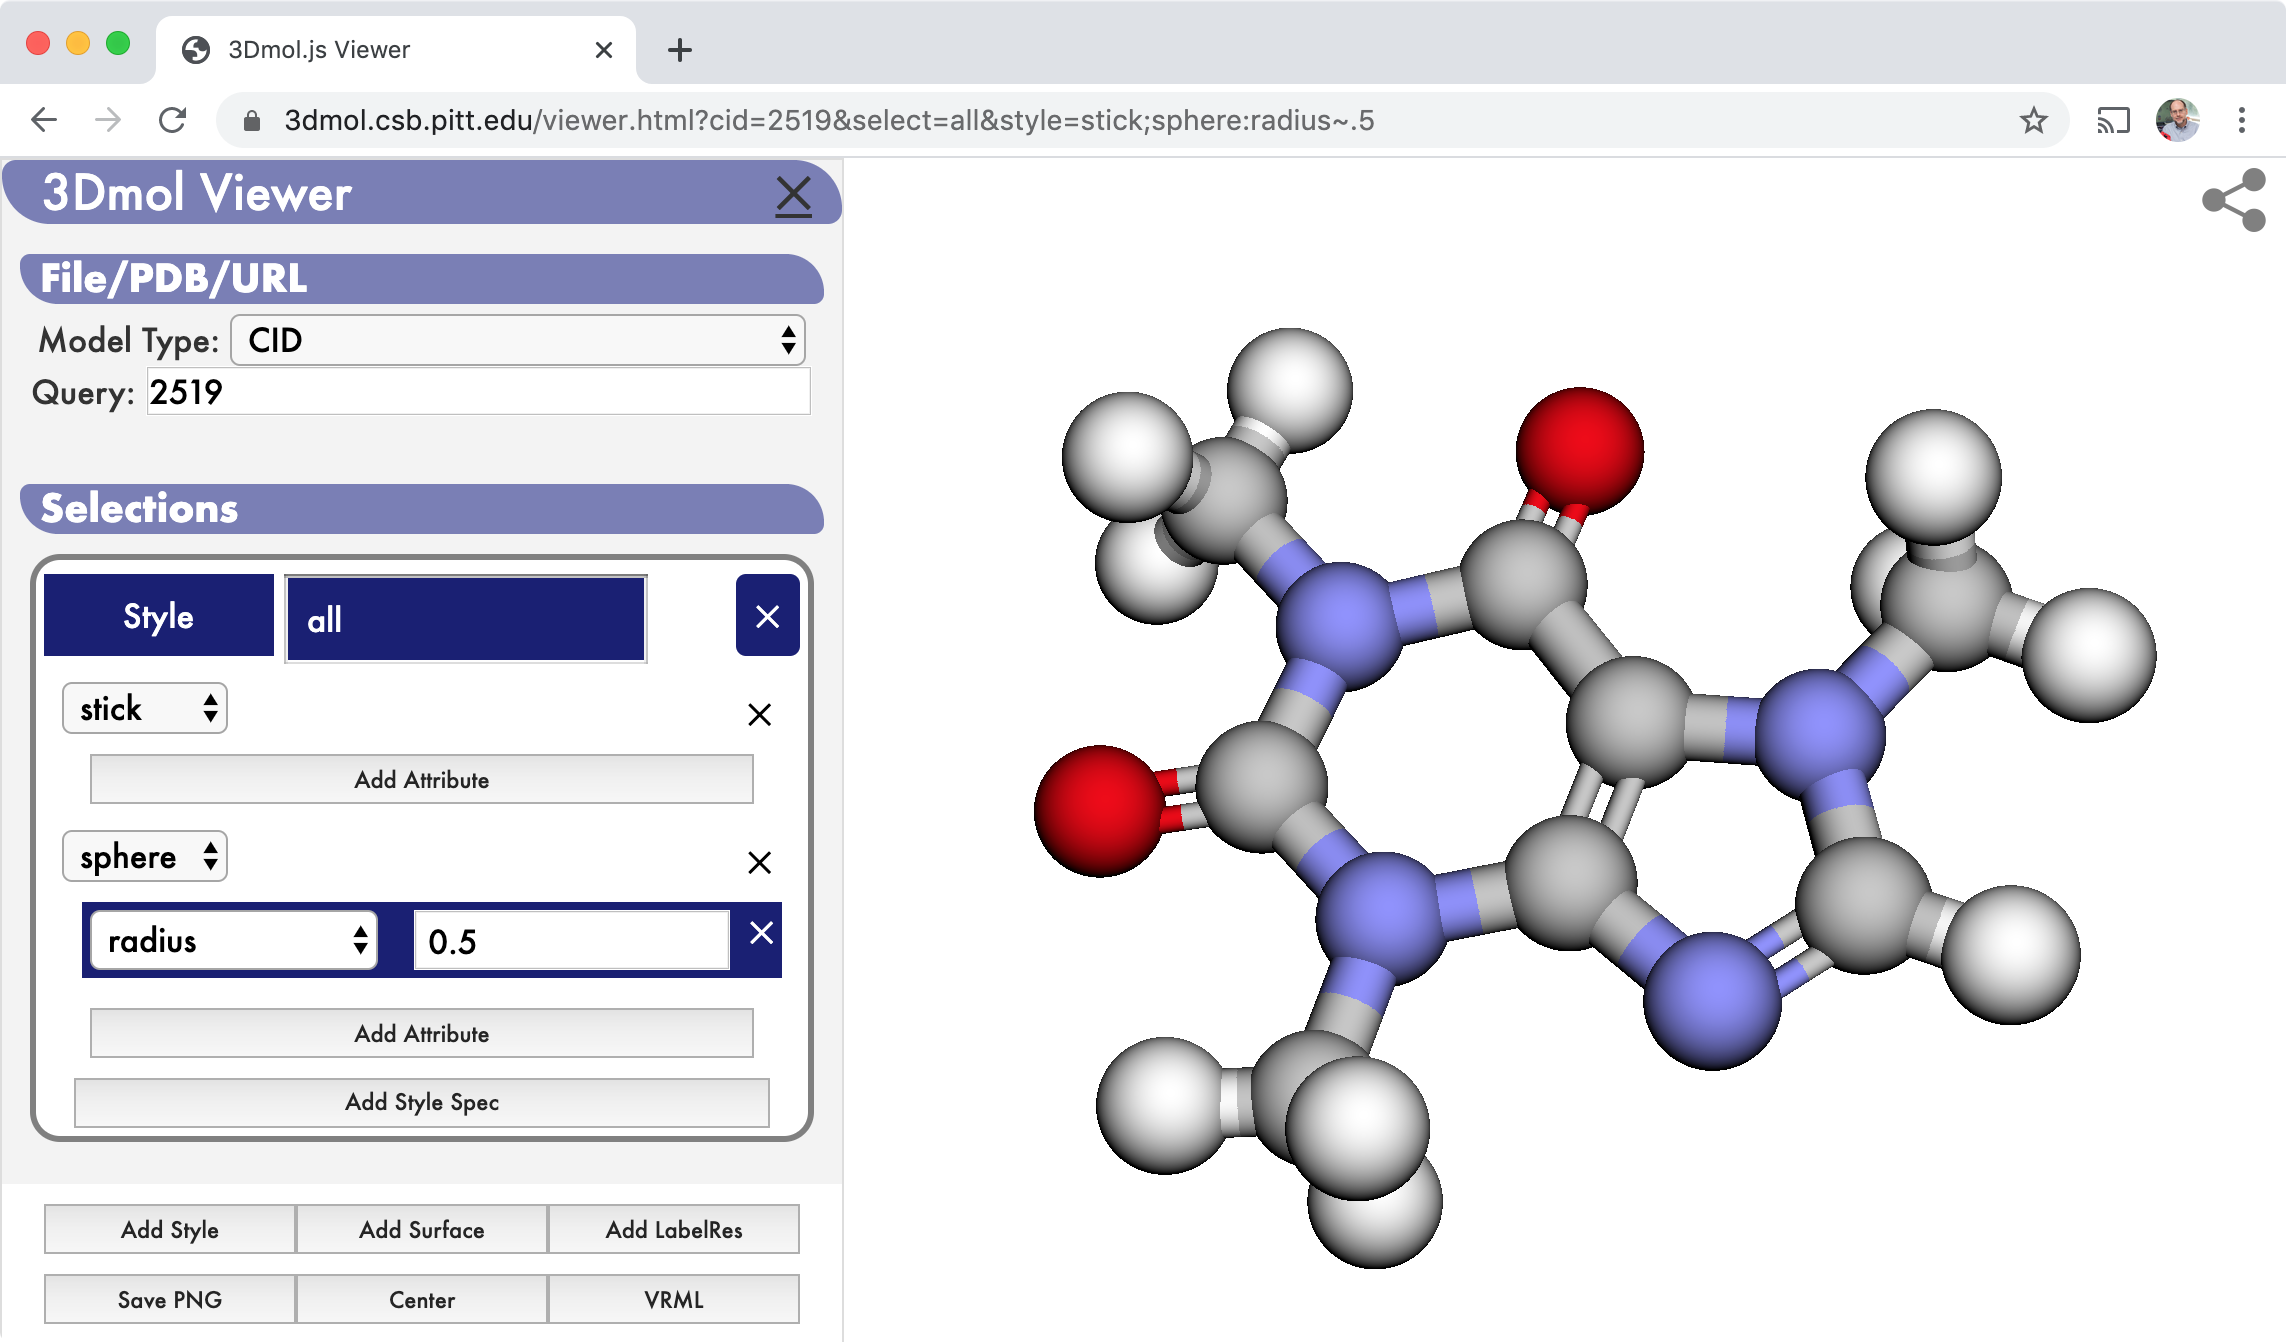
\includegraphics[width=\linewidth]{viewer}
    \caption{The 3Dmol.js viewer.  The edit panel (left) is shown and is used to load a molecule, in this case compound id 2519 from PubChem, and set the style.  The result can be accessed at the URL \url{https://3dmol.csb.pitt.edu/viewer.html?cid=2519&select=all&style=stick;sphere:radius~.5}}
    \label{fig:viewer}
\end{figure}

\section{3Dmol.js Classroom Response System}

3Dmol.js\cite{rego20153dmol} is a WebGL-based JavaScript library for hardware-accelerated online molecular graphics.  It supports most molecular file formats and visualization styles, including support for volumetric data (e.g. cube files) and simulation data (e.g. AMBER\cite{case2005amber} or GROMACS\cite{van2005gromacs} data).  In addition to its full-featured JavaScript API, 3Dmol.js offers an embedding API, where a molecular view can be added to a web page by inserting a single \texttt{div} statement, and a URL-based hosted viewer API. The hosted viewer (\url{http://3dmol.csb.pitt.edu/viewer.html}) is specifically designed so that all information to display the current molecular view is included in the URL.  That is, having constructed a scene by loading the appropriate molecular data and applying the desired styles using the provided edit panel (Figure~\ref{viewer}), it is possible to share the URL with students (e.g. as a QR code) so they can see the identical scene and interact with it.  As 3Dmol.js is open source (BSD License), instructors may host the viewer on their own web servers if desired.  We have added functionality to the 3Dmol.js API and hosted viewer to enable its use as a classroom response system where students answer queries by clicking on atoms of a 3D molecule.

\begin{figure}
    \centering
    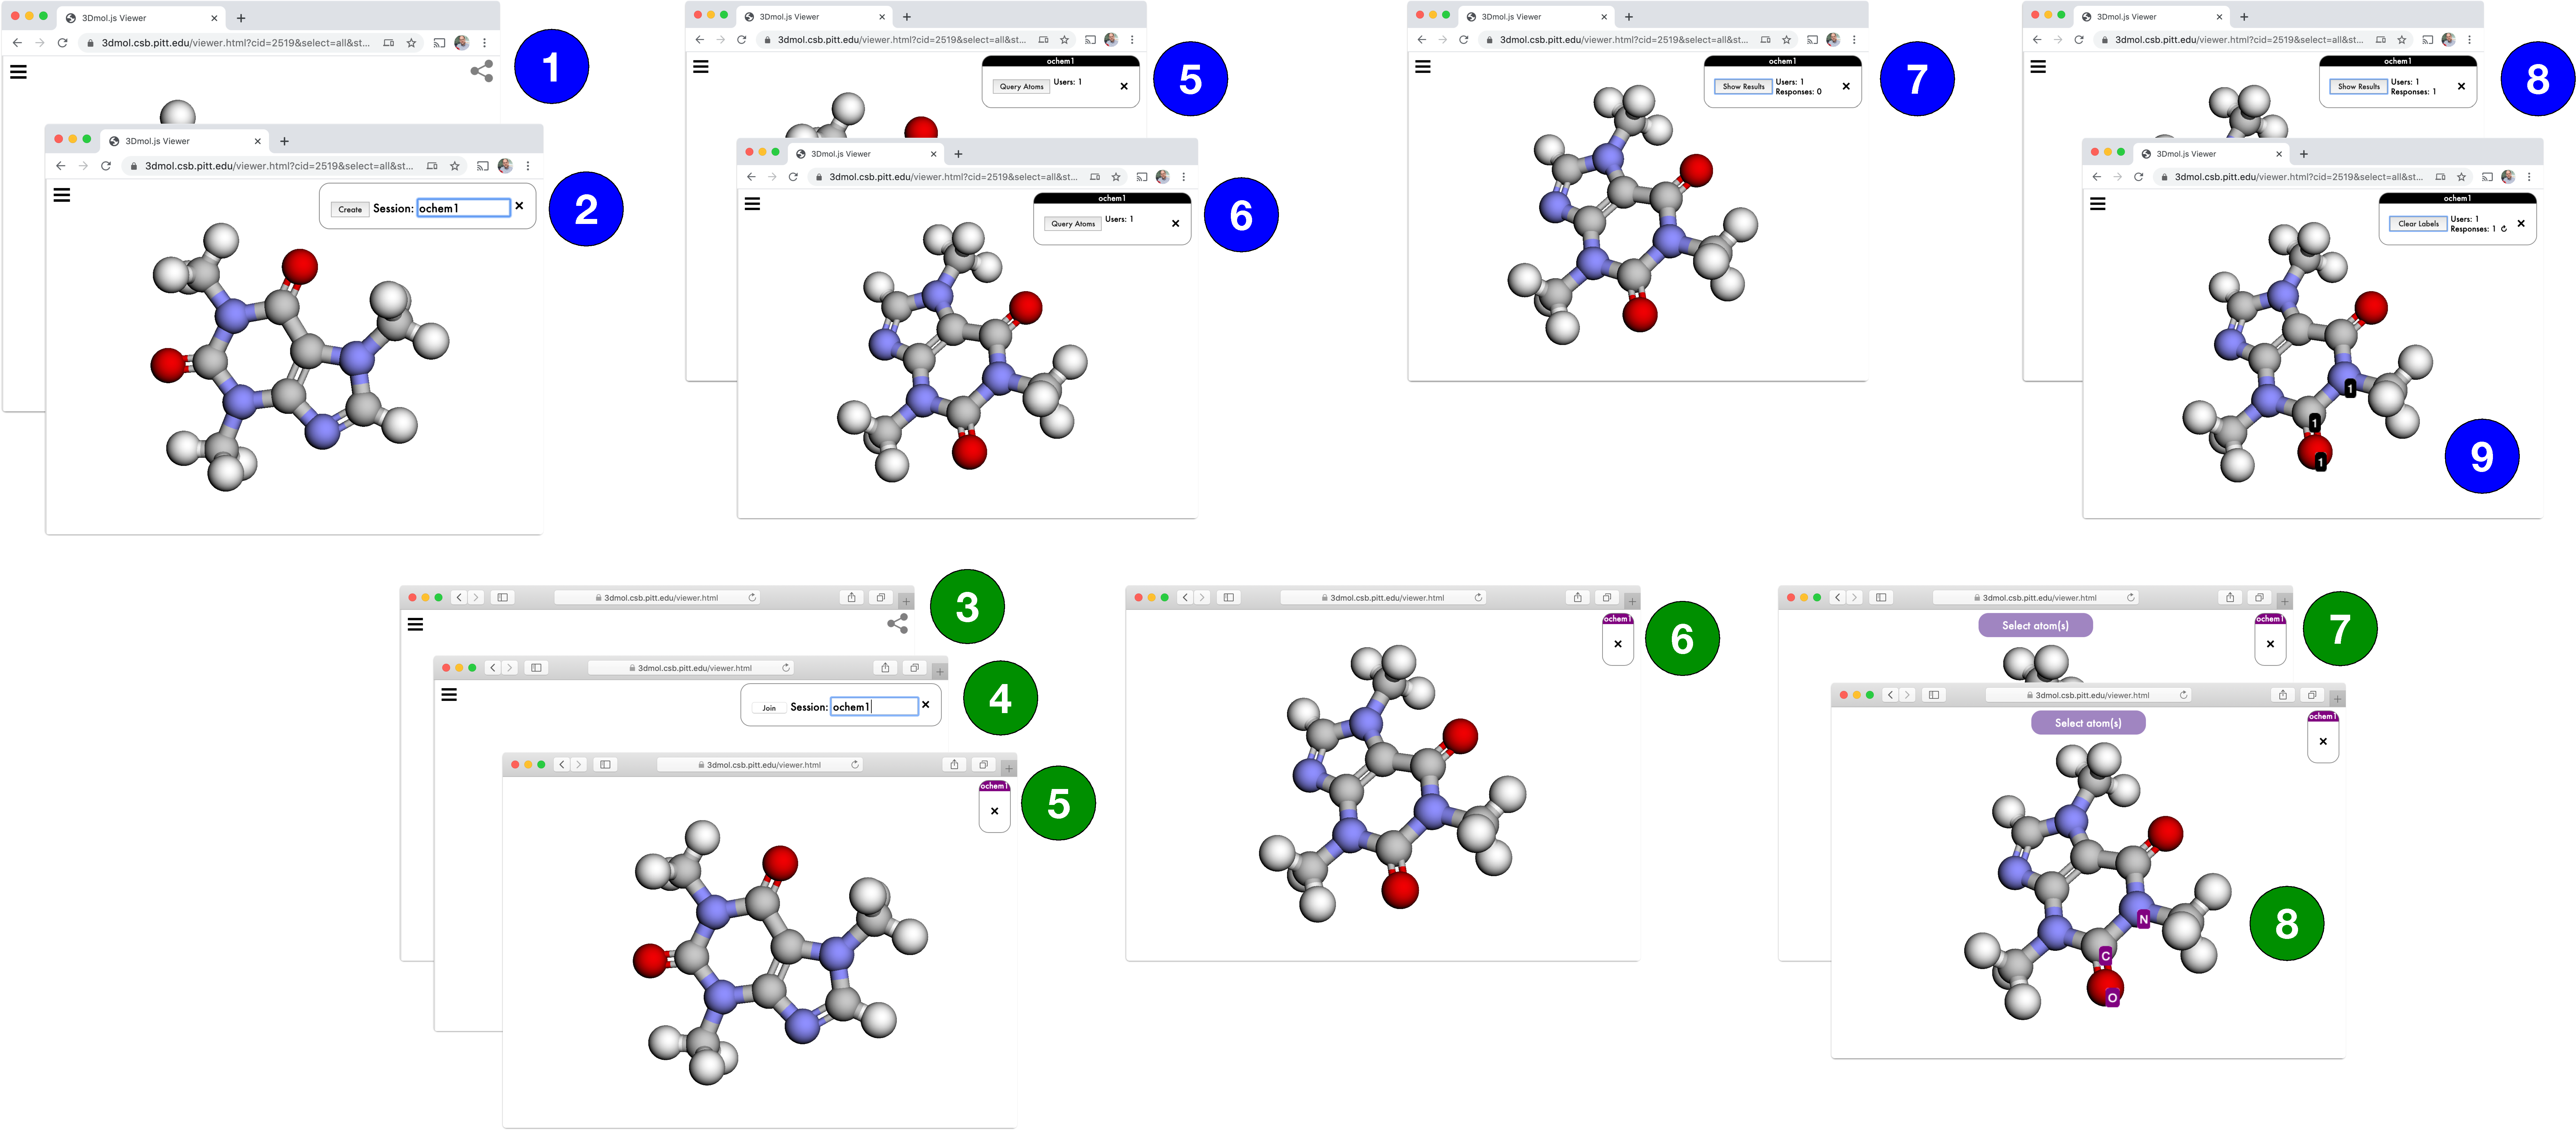
\includegraphics[width=\linewidth]{flow}
    \caption{Flow of instructor (top) and student (bottom) interactions with the 3Dmol.js classroom response system.}
    \label{fig:flow}
\end{figure}

\subsection{User Interface}

Usage of the classroom response features are shown in Figure~\ref{fig:flow}.  (1) The instructor clicks on the `share' icon in the upper right of the hosted viewer. (2) In the resulting text box, the instructor creates a session by specifying its name.  Once created, a session lasts as long as the creating browser window is left open and only that browser window has the ability to manipulate the session contents.  The session will be initialized with the current molecular view. If a session is already available, the `Create' button will change to a `Join' button.  (3) When students click on the share button (4) they enter the name of the already created session and click `Join.'  (5) This populates their viewer with the instructor's molecular view and the instructor's view is updated to show that an additional user has connected.  Monitoring the number of connections is important for ensuring the whole class is participating.  (6) When the instructor modifies the view of the molecule the student's view is updated to match.  As long as the instructor is not changing the view, students can freely interact with the molecule by rotating, translating, or zooming the view.


\subsection{Implementation}

technical details, how to use

\section{Case Study}

Description and pictures of how recitation was conducted.

\section{Discussion}

open source, availability, future plans: grid (multi-molecule) view, integration with jupyter notebooks, file upload, volumetric data

%%%%%%%%%%%%%%%%%%%%%%%%%%%%%%%%%%%%%%%%%%%%%%%%%%%%%%%%%%%%%%%%%%%%%
%% The "Acknowledgement" section can be given in all manuscript
%% classes.  This should be given within the "acknowledgement"
%% environment, which will make the correct section or running title.
%%%%%%%%%%%%%%%%%%%%%%%%%%%%%%%%%%%%%%%%%%%%%%%%%%%%%%%%%%%%%%%%%%%%%
\begin{acknowledgement}



The authors thank.. 

\end{acknowledgement}

%%%%%%%%%%%%%%%%%%%%%%%%%%%%%%%%%%%%%%%%%%%%%%%%%%%%%%%%%%%%%%%%%%%%%
%% The same is true for Supporting Information, which should use the
%% suppinfo environment.
%%%%%%%%%%%%%%%%%%%%%%%%%%%%%%%%%%%%%%%%%%%%%%%%%%%%%%%%%%%%%%%%%%%%%
%\begin{suppinfo}
%\end{suppinfo}

%%%%%%%%%%%%%%%%%%%%%%%%%%%%%%%%%%%%%%%%%%%%%%%%%%%%%%%%%%%%%%%%%%%%%
%% The appropriate \bibliography command should be placed here.
%% Notice that the class file automatically sets \bibliographystyle
%% and also names the section correctly.
%%%%%%%%%%%%%%%%%%%%%%%%%%%%%%%%%%%%%%%%%%%%%%%%%%%%%%%%%%%%%%%%%%%%%
\bibliography{references}

\end{document}